\section{Matrices and Linear Transformations}

\subsection{Rotation matrices}\label{sec:rotation-matrices}

Make stuff spin around!

\subsubsection{Two dimensional}

\begin{figure}[H]
\centering
    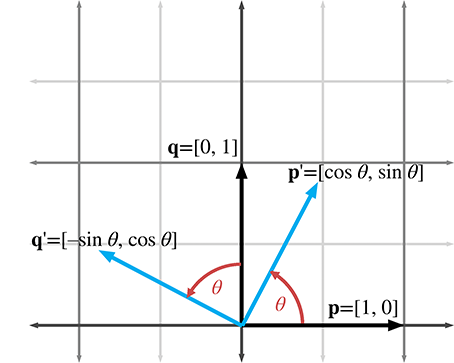
\includegraphics{05_2d_rotation}
\caption{2D rotation visualization}
\label{fig:2d-rotation-visualization}
\end{figure}

$$
\begin{matrix}
{\mathbf{R}(\theta) =
\begin{bmatrix}
{\cos\theta} & {\sin\theta} \\
{- \sin\theta} & {\cos\theta} \\
\end{bmatrix}.} \\
\end{matrix}
$$

\subsubsection{Three dimensional}

Rotation around x-axis: \\
$$
\mathbf{R}_{x}(\theta) = 
\mathbf{R}(
\begin{bmatrix}
1 & 0 & 0 
\end{bmatrix},
\theta) =
 \begin{bmatrix}
1 & 0 & 0 \\
0 & {\cos\theta} & {\sin\theta} \\
0 & {- \sin\theta} & {\cos\theta} \\
\end{bmatrix}
$$

Rotation around y-axis: \\
$$
\mathbf{R}_{y}(\theta) = 
\mathbf{R}(
\begin{bmatrix}
0 & 1 & 0 
\end{bmatrix},
\theta) = \begin{bmatrix}
{\cos\theta} & 0 & {- \sin\theta} \\
0 & 1 & 0 \\
{\sin\theta} & 0 & {\cos\theta} \\
\end{bmatrix}
$$

Rotation around z-axis: \\
$$
\mathbf{R}_{z}(\theta) =
\mathbf{R}(
\begin{bmatrix}
0 & 0 & 1
\end{bmatrix},
\theta) =
\begin{bmatrix}
{\cos\theta} & {\sin\theta} & 0 \\
{- \sin\theta} & {\cos\theta} & 0 \\
0 & 0 & 1 \\
\end{bmatrix}
$$

Rotation around arbitrary axis: \\
$$
\mathbf{R}(\hat{\mathbf{n}},\theta) =
\begin{bmatrix}
{{n_{x}}^{2}\left( 1 - \cos\theta \right) + \cos\theta} & {n_{x}n_{y}\left( 1 - \cos\theta \right) + n_{z}\sin\theta} & {n_{x}n_{z}\left( 1 - \cos\theta \right) - n_{y}\sin\theta} \\
{n_{x}n_{y}\left( 1 - \cos\theta \right) - n_{z}\sin\theta} & {{n_{y}}^{2}\left( 1 - \cos\theta \right) + \cos\theta} & {n_{y}n_{z}\left( 1 - \cos\theta \right) + n_{x}\sin\theta} \\
{n_{x}n_{z}\left( 1 - \cos\theta \right) + n_{y}\sin\theta} & {n_{y}n_{z}\left( 1 - \cos\theta \right) - n_{x}\sin\theta} & {{n_{z}}^{2}\left( 1 - \cos\theta \right) + \cos\theta} \\
\end{bmatrix}
$$

Note that the standard matrices for $x$-, $y$- and $z$-axis can be computed by replacing $\hat{\textbf{n}}$ with the corresponding basis vector. See exercise 2.24. Furthermore, check the book if you want to understand how to derrive these rotation matrices.

\subsection{Scaling matrices}

With scaling can make objects bigger or smaller. When all axes are scaled equally we are scaling \textit{uniformly}, otherwise it's called \textit{non-uniform} scaling.

\subsubsection{Two dimensional}

\begin{figure}[H]
\centering
    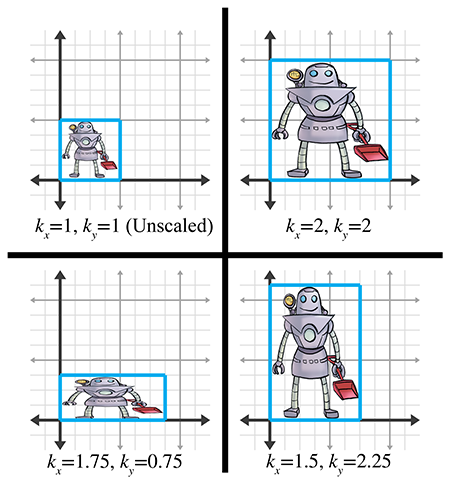
\includegraphics{05_scaling}
\caption{2D scaling}
\label{fig:2d-scaling}
\end{figure}

Scaling along the cardinal axes: \\
$$
\mathbf{S}(k_{x},k_{y}) =
\begin{bmatrix}
k_{x} & 0 \\
0 & k_{y} \\
\end{bmatrix}
$$

\subsubsection{Three dimensional}

Scaling along the cardinal axes: \\
$$
\mathbf{S}(k_{x},k_{y},k_{z}) = 
\begin{bmatrix}
k_{x} & 0 & 0 \\
0 & k_{y} & 0 \\
0 & 0 & k_{z}
\end{bmatrix}
$$

Scaling along an arbitrary vector: \\
$$
\mathbf{S}(\hat{\mathbf{n}},k) = \begin{bmatrix}
{1 + \left( k - 1 \right){n_{x}}^{2}} & {\left( k - 1 \right)n_{x}n_{y}} & {\left( k - 1 \right)n_{x}n_{z}} \\
{\left( k - 1 \right)n_{x}n_{y}} & {1 + \left( k - 1 \right){n_{y}}^{2}} & {\left( k - 1 \right)n_{y}n_{z}} \\
{\left( k - 1 \right)n_{x}n_{z}} & {\left( k - 1 \right)n_{y}n_{z}} & {1 + \left( k - 1 \right){n_{z}}^{2}} \\
\end{bmatrix}
$$

As an execise try scaling along the $x$-axis with a factor of $5$, that is $\mathbf{S}(
\begin{bmatrix}
1 & 0 & 0
\end{bmatrix},5)$. It will all make sense, or maybe not.

\subsection{Orthographic projection}

\begin{figure}[H]
\centering
    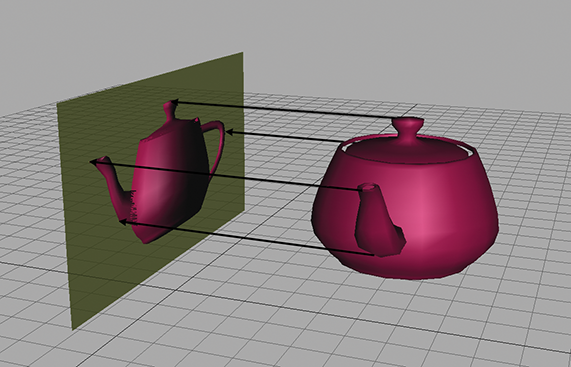
\includegraphics{05_projection}
\caption{2D projection}
\label{fig:2d-projection}
\end{figure}

The term \textit{projection} in general refers to any dimension reducing operation, so essentially we are going to discard some coordinate. This means we can scale some arbitrary vector by a scale of\dots $0$. No new derivations or matrices, simply use $\mathbf{S}(\hat{\mathbf{n}},0)$.

\subsection{Reflection}

\begin{figure}[H]
\centering
    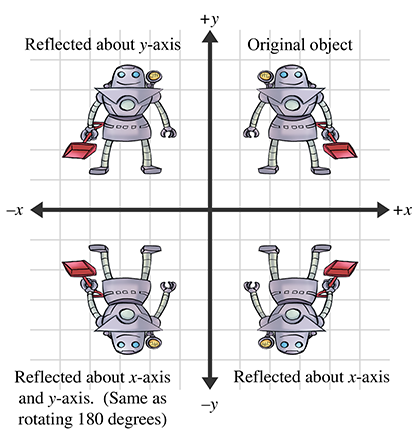
\includegraphics{05_reflection}
\caption{2D reflection}
\label{fig:2d-reflection}
\end{figure}

Reflection is flipping some axis once, that is, multiplying by $-1$. We once again use our scaling matrices, but this time with a value of $-1$. We can apply a reflection to any arbitrary vector as follows: $\mathbf{S}(\hat{\mathbf{n}},-1)$.

\subsection{Shearing}

\begin{figure}[H]
\centering
    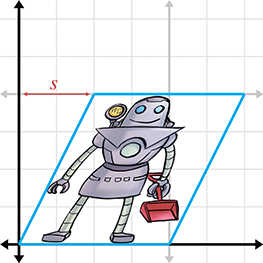
\includegraphics{05_shearing}
\caption{2D shearing}
\label{fig:2d-shearing}
\end{figure}

Shearing also known as skewing basically distorts the coordinate space as shown in the picture above. Check the book for the matrices as this transformation is seldom used, but you know, it's good to know it exists.
